%\section{Une section}

% remarque : pour qu'un mot se retrouve dans le lexique : \MotDefinition{asymptote horizontale}{} 

\begin{aconnaitre}
La \MotDefinition{fraction}{} $\dfrac{a}{\textcolor{C1}{b}}$ est le quotient de l'entier relatif $a$ par l'entier relatif $\textcolor{C1}{b}$ (avec $\textcolor{C1}{b} \neq 0$), ainsi :

$\dfrac{a}{\textcolor{C1}{b}} = a : \textcolor{C1}{b}$. Le nombre $a$ s'appelle le \MotDefinition{numérateur}{}, $\textcolor{C1}{b}$ est le \MotDefinition{dénominateur}{} et le trait horizontal est la \MotDefinition{barre de fraction}{}. Un nombre \MotDefinition{rationnel}{} est un nombre qui peut s'écrire comme une fraction.
\end{aconnaitre}


\begin{methode*1}[Utiliser la définition du quotient]

\begin{exemple*1}
Parmi les nombres suivants : $\dfrac{3}{4}$  ; $\dfrac{23}{2,3}$ ; $\dfrac{13}{15}$ ; $\dfrac{0}{10}$ ;   $\dfrac{1,2}{5}$, détermine ceux qui ne sont pas une fraction.

\vspace{.5em}

Une fraction possède un numérateur \textbf{et} un dénominateur entier. Donc $\dfrac{23}{2,3}$ et $\dfrac{1,2}{5}$ ne sont pas des fractions.
 \end{exemple*1}
 
\begin{remarque}
{\footnotesize Les quotients $\dfrac{23}{2,3}$, $\dfrac{1,2}{5}$ utilisent l'écriture fractionnaire mais ne sont pas des fractions. Par contre ce sont des nombres rationnels car $\dfrac{23}{2,3} = 10$ et $\dfrac{1,2}{5} = 0,24$.}
 \end{remarque}
 
  \exercice  
Parmi les expressions suivantes, barre celles qui ne sont pas des fractions :
$\dfrac{-2}{1}$  ; $\dfrac{1,7}{1,7}$ ; $\dfrac{10}{0}$ ; $\dfrac{0}{-8}$ ;   $\dfrac{-3,01}{5}$
%\correction

 \end{methode*1}

%%%%%%%%%%%%%%%%%%%%%%%%%%%%%%%%%%%%%%%%%%%%%%%%%%%%%%%%%%%%%%%%%%

\begin{aconnaitre}
Une \MotDefinition{fraction décimale}{} est une fraction dont le dénominateur est 1, 10, 100, 1\,000 \ldots
Un nombre pouvant s'écrire sous la forme d'une fraction décimale est un \MotDefinition{nombre décimal}{}. Il peut aussi se noter en utilisant une virgule ; c'est son \MotDefinition{écriture décimale}{}.
\end{aconnaitre}

\begin{methode*1}[Utiliser les fractions décimales]

\begin{exemple*1}
Donne l'écriture décimale du nombre $\dfrac{567}{10}$ :\\[0.5em]
L'écriture décimale est obtenue en calculant la division $567 : 10 = 56,7$.
 \end{exemple*1}
 
\begin{exemple*1}
Écris 0,25 sous la forme d'une fraction décimale. \\[0.5em]
Une fraction décimale a pour dénominateur 1, 10, 100, 1\,000, \ldots .

Le chiffre 5 occupe la position des centièmes.

On obtient la fraction décimale $0,25 = \dfrac{25}{100}$.
 \end{exemple*1}
 
  \exercice
Donne l'écriture décimale des nombres :
\vspace{.8em}
\begin{colenumerate}{3}
 \item $\dfrac{12}{5}$ \dotfill;
 \item $\dfrac{2,5}{2}$ \dotfill;
 \item $\dfrac{4}{2,5}$\dotfill.
 \end{colenumerate}
%\correction

  \exercice
Écris les nombres suivants sous la forme d'une fraction décimale :
\vspace{.8em}
\begin{colenumerate}{3}
 \item $0,8$ \dotfill;
 \item $0,12$ \dotfill;
 \item $1,541$\dotfill.
 \end{colenumerate}
%\correction

 \end{methode*1}

%%%%%%%%%%%%%%%%%%%%%%%%%%%%%%%%%%%%%%%%%%%%%%%%%%%%%%%%%%%%%%%%%%

\begin{methode*1}[Fraction d'un tout]

\begin{exemple*1}
\begin{minipage}[c]{0.4\linewidth}
Détermine quelle fraction de la figure est colorée.
 \end{minipage} \hfill%
 \begin{minipage}[c]{0.4\linewidth}
 \scalebox{.5}{
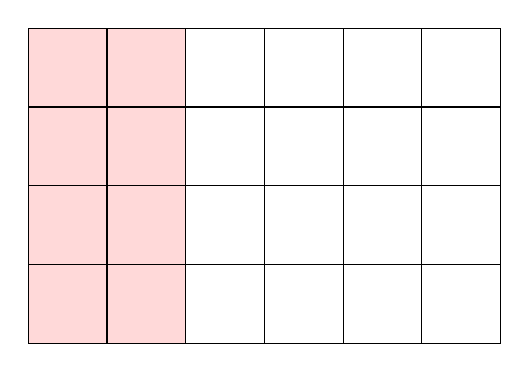
\begin{tikzpicture}	
  
    
\def \CharSize {1};
\def \BulletSize {1};

%la partie colorée
\draw [fill=pink!60](0,0) rectangle (2,4);
%la grille
\draw (0,0) grid (6,4);

\end{tikzpicture} 
 } %fin de la scalebox
 \end{minipage} \\[1em]
La figure est divisée en 24 parties identiques et 8 sont colorées. On a coloré les $\dfrac{8}{24}$ de la figure.
 \end{exemple*1}
 
\begin{remarque}
La division de la figure aurait pu être en 12 parties identiques dont 4 sont colorées, c'est-à-dire, $\dfrac{4}{12}$ de la figure ou les $\dfrac{2}{6}$ de la figure ou les $\dfrac{1}{3}$ de la figure. Mais toutes ces fractions sont égales.
 \end{remarque}

  \exercice
Pour chaque figure donne la fraction de la partie colorée :
\begin{colenumerate}{3}
 \item 
 
 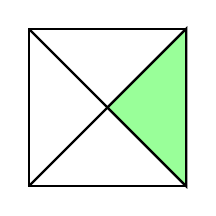
\begin{tikzpicture}	
  
    
\def \CharSize {1};
\def \BulletSize {1};


\draw[thick] (0,0)--(2,0)--(2,2)--(0,2)--cycle;
\draw[thick] (0,2)--(2,0);
\draw[thick] (0,0)--(2,2);
\draw[thick,fill=green!40] (2,0)--(1,1)--(2,2)--cycle;

\end{tikzpicture} 

 \item 
 
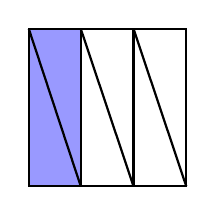
\begin{tikzpicture}	
  
    
\def \CharSize {1};
\def \BulletSize {1};

%carré
\draw[thick] (0,0)--(2,0)--(2,2)--(0,2)--cycle;
%verticales
\draw[thick] (0.66,0)--(0.66,2);
\draw[thick] (1.33,0)--(1.33,2);
%partie colorée
\draw[thick,fill=blue!40] (0,0)--(0.66,0)--(0.66,2)--(0,2)--cycle;
%obliques
\draw[thick] (0,2)--(0.66,0);
\draw[thick] (0.66,2)--(1.33,0);
\draw[thick] (1.33,2)--(2,0);


\end{tikzpicture}
 \item 
 
 \scalebox{.5}{
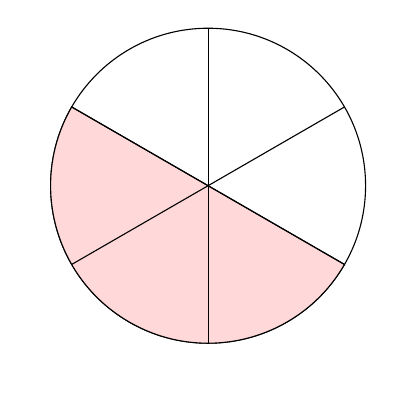
\begin{tikzpicture}	
  
%le cercle
\draw (0,0) circle (2);
%le secteur coloré
\draw [fill=pink!60](0,0)--(150:2) arc(150:330:2)--cycle;

%les secteurs
   \foreach \a in {30,90,150}{\draw (\a:-2)--(\a:2);}

\end{tikzpicture} 
 } %fin de la scalebox
 \end{colenumerate}  
%\correction

 \end{methode*1}

%%%%%%%%%%%%%%%%%%%%%%%%%%%%%%%%%%%%%%%%%%%%%%%%%%%%%%%%%%%%%%%%%%

\begin{methode*1}[Placer le quotient de deux entiers sur une demi‑droite graduée]

\begin{exemple*1}
Place sur une même demi‑droite graduée les points $A$ et $B$ d'abscisses respectives $\dfrac{5}{6}$ et $\dfrac{11}{3}$. \\[1em]
On choisit une longueur unité $OI$ que l'on partage en six parts égales. Chacune de ces parts correspond donc à \textcolor{C1}{$\dfrac{1}{6}$} de l'unité.
\begin{itemize}
 \item Pour placer le point $A$, on utilise $\dfrac{5}{6} = 5 \cdot \dfrac{1}{6}$ et on reporte donc cinq \textcolor{C1}{sixièmes} à partir du point $O$.
 \begin{center} 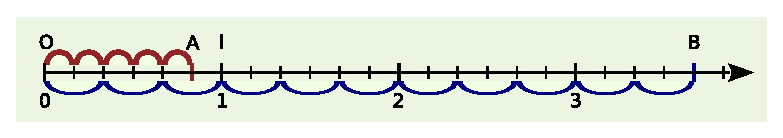
\includegraphics[width=10cm]{quotient_ddroite} \end{center}
 \item Pour placer le point $B$, on remarque que deux parts correspondent à $\dfrac{1}{3}$ de l'unité et on utilise $\dfrac{11}{3} = 11 \cdot \dfrac{1}{3}$. On reporte donc 11 tiers à partir du point $O$.
 \end{itemize}
 \end{exemple*1}
 
 
 \exercice
 Sur une même demi‑droite graduée, place les points $E \bigg(\dfrac{3}{4} \bigg)$ ; $F \bigg(2 - \dfrac{1}{4} \bigg)$ et $G \bigg(\dfrac{5}{2} \bigg)$.
%\correction

 \end{methode*1}

%%%%%%%%%%%%%%%%%%%%%%%%%%%%%%%%%%%%%%%%%%%%%%%%%%%%%%%%%%%%%%%%%%

\begin{aconnaitre}
Un quotient ne change pas quand on \textbf{multiplie} ou qu'on \textbf{\textcolor{A1}{divise}} son numérateur et son dénominateur par un \textbf{même nombre} non nul :
\begin{center} $\dfrac{a}{b} = \dfrac{a \cdot \textcolor{C1}{k}}{b \cdot \textcolor{C1}{k}}$ ou $\dfrac{a}{b} = \dfrac{a : \textcolor{C1}{k}}{b : \textcolor{C1}{k}}$ où $a$, $b$ et $k$ sont des nombres, avec $b \neq 0$ et $k \neq 0$. \end{center}
\end{aconnaitre}


\begin{methode*1}[Reconnaître des écritures fractionnaires égales]

\begin{exemple*1}
Montre que $\dfrac{5}{7}$ et $\dfrac{40}{56}$ représentent un même nombre. \\[1em]
On sait que $5 \cdot \text{\textbf{\textcolor{C2}{8}}} = 40$ et que $7 \cdot \text{\textbf{\textcolor{C2}{8}}} = 56$. 
En multipliant le numérateur et le dénominateur par le même nombre, on obtient $\dfrac{5}{7} = \dfrac{5 \cdot \text{\textbf{\textcolor{C2}{8}}}}{7 \cdot \text{\textbf{\textcolor{C2}{8}}}} = \dfrac{40}{56}$, ce qui signifie que $\dfrac{5}{7}$ et $\dfrac{40}{56}$ représentent le même nombre.
 \end{exemple*1}
 
 \begin{exemple*1}
Parmi  $\dfrac{21}{27}$ ; $\dfrac{56}{81}$ ; $\dfrac{0,7}{0,9}$ ; $\dfrac{48}{63}$ et $\dfrac{23,1}{29,7}$ relève les nombres égaux à $\dfrac{7}{9}$. \\[1em]
\begin{itemize}
 \item $\dfrac{7}{9} = \dfrac{7 \cdot \text{\textbf{\textcolor{C2}{3}}}}{9 \cdot \text{\textbf{\textcolor{C2}{3}}}} = \dfrac{21}{27}$ donc $\dfrac{7}{9} = \dfrac{21}{27}$ ;
\vspace{0.3cm}
\item $\dfrac{0,7}{0,9} = \dfrac{0,7 \cdot \text{\textbf{\textcolor{C2}{10}}}}{0,9 \cdot \text{\textbf{\textcolor{C2}{10}}}} = \dfrac{7}{9}$ donc $\dfrac{7}{9} = \dfrac{0,7}{0,9}$ ;
  \item On remarque que $7 \cdot \text{\textbf{\textcolor{C2}{8}}} = 56$ et que $9 \cdot 8 = 72$ donc $\dfrac{7}{9} = \dfrac{7 \cdot \text{\textbf{\textcolor{C2}{8}}}}{9 \cdot \text{\textbf{\textcolor{C2}{8}}}} = \dfrac{56}{72}$ et $\dfrac{7}{9} \neq \dfrac{56}{81}$;
  \item On remarque que $9 \cdot \text{\textbf{\textcolor{C2}{7}}} = 63$ et que $7 \cdot 7 = 49$ donc $\dfrac{7}{9} = \dfrac{7 \cdot \text{\textbf{\textcolor{C2}{7}}}}{9 \cdot \text{\textbf{\textcolor{C2}{7}}}} = \dfrac{49}{63}$ et $\dfrac{7}{9} \neq \dfrac{48}{63}$ ; 
 \vspace{0.3cm}
  \item On détermine le nombre qui multiplié par 7 donne 23,1. Ce nombre est $\dfrac{23,1}{7}$. En effectuant la division, on trouve $23,1 : 7 = 3,3$.

Or $9 \cdot 3,3 = 29,7$ donc $\dfrac{7}{9} = \dfrac{7 \cdot \text{\textbf{\textcolor{C2}{3,3}}}}{9 \cdot \text{\textbf{\textcolor{C2}{3,3}}}} = \dfrac{23,1}{29,7}$.
 \end{itemize}
Les écritures fractionnaires de la liste égales à $\dfrac{7}{9}$ sont donc $\dfrac{21}{27}$ ; $\dfrac{0,7}{0,9}$ ; $\dfrac{23,1}{29,7}$.
 \end{exemple*1}
 
 
  \exercice
Parmi les nombres $\dfrac{45}{27}$ ; $\dfrac{0,05}{0,03}$ ; $\dfrac{54}{33}$ ; $\dfrac{90}{54}$ et $\dfrac{40}{25}$ relève ceux qui sont

égaux à $\dfrac{5}{3}$.
%\correction

  \exercice
  Trouve une fraction égale à chaque fraction de la liste $\dfrac{40}{90}$ ; $\dfrac{18}{72}$ ; $\dfrac{16}{24}$ et $\dfrac{125}{75}$.
%\correction

 \end{methode*1}

%%%%%%%%%%%%%%%%%%%%%%%%%%%%%%%%%%%%%%%%%%%%%%%%%%%%%%%%%%%%%%%%%%

\begin{aconnaitre}
\MotDefinition{Amplifier une fraction}{} consiste à obtenir une fraction égale en multipliant le numérateur et le dénominateur par le même nombre entier non nul. \\[0.5em]
\MotDefinition{Simplifier ou réduire une fraction}{} consiste à obtenir une fraction égale en divisant le numérateur et le dénominateur par le même nombre entier non nul. \\[0.5em]
Une \MotDefinition{fraction irréductible}{} est une fraction qu'on ne peut plus simplifier.
\end{aconnaitre}


\begin{methode*1}[Simplifier une fraction]

\begin{exemple*1}
Rends la fraction $\dfrac{48}{60}$ irréductible. \\[1em]
On utilise les critères de divisibilité connus et les tables de multiplication :
\begin{itemize}
 \item Le chiffre des unités de 48 est 8 et celui de 60 est 0 donc 48 et 60 sont divisibles par 2. 
Ainsi $\dfrac{48}{60} = \dfrac{\text{\textbf{\textcolor{C2}{2}}} \cdot 24}{\text{\textbf{\textcolor{C2}{2}}} \cdot 30} = \dfrac{24}{30}$ On dit qu'on a \textbf{simplifié} la fraction $\dfrac{48}{60}$ par 2.
 \item On remarque que 24 et 30 sont des multiples de 6. On peut donc encore simplifier la fraction par 6.
 Ainsi $\dfrac{24}{30} = \dfrac{\text{\textbf{\textcolor{C2}{6}}} \cdot 4}{\text{\textbf{\textcolor{C2}{6}}} \cdot 5} = \dfrac{4}{5}$.
 \end{itemize}
Une fraction plus simple égale à $\dfrac{48}{60}$ est donc par exemple $\dfrac{24}{30}$ ou encore $\dfrac{4}{5}$.
$\dfrac{4}{5}$ n'est plus simplifiable. C'est la fraction irréductible égale à $\dfrac{48}{60}$.
 \end{exemple*1}
 
\begin{exemple*1}
Écris 2,5 sous la forme d'une fraction irréductible : \\[1em]
$2,5 = \dfrac{25}{10} = \dfrac{5 \cdot \text{\textbf{\textcolor{C2}{5}}}}{2 \cdot \text{\textbf{\textcolor{C2}{5}}}} = \dfrac{5}{2}$.
 \end{exemple*1}
 
 
  \exercice
Rends irréductible les fractions : $\dfrac{27}{36}$, $\dfrac{75}{30}$, $\dfrac{45}{39}$.
%\correction

  \exercice
Simplifie $\dfrac{20}{12}$ puis trouve un quotient égal dont le dénominateur est 21.
%\correction

  \exercice
Écris les nombres suivants sous la forme d'une fraction irréductible :
\begin{colenumerate}{3}
 \item 0,5 \dotfill;
 \item 1,5 \dotfill;
 \item 0,8 \dotfill.
 \end{colenumerate}
%\correction

 \end{methode*1}

%%%%%%%%%%%%%%%%%%%%%%%%%%%%%%%%%%%%%%%%%%%%%%%%%%%%%%%%%%%%%%%%%%

%%%%%%%%%%%%%%%%%%%%%%%%%%%%%%%%%%%
%%%%%%%%%%%%%%%%%%%%%%%%%%%%%%%%%%%
%MiseEnPage
%%%%%%%%%%%%%%%%%%%%%%%%%%%%%%%%%%%
\newpage
%%%%%%%%%%%%%%%%%%%%%%%%%%%%%%%%%%%
%%%%%%%%%%%%%%%%%%%%%%%%%%%%%%%%%%%


\begin{aconnaitre}
Pour \MotDefinition{comparer des nombres en écriture fractionnaire}{}, on les écrit avec le même dénominateur, puis on les range dans le même ordre que leurs numérateurs. \\[0.5em]
Si le numérateur d'un nombre en écriture fractionnaire est supérieur à son dénominateur, alors il est supérieur à 1. Si son numérateur est inférieur à son dénominateur alors il est inférieur à 1.
\end{aconnaitre}


\begin{methode*1}[Comparer]

\begin{exemple*1}
Compare les fractions $\dfrac{12}{4}$ et $\dfrac{57}{20}$ :
\begin{center}
 \begin{tabularx}{\linewidth}{ccX}
  $\dfrac{12}{4} = \dfrac{12 \cdot \text{\textbf{\textcolor{C2}{5}}}}{4 \cdot \text{\textbf{\textcolor{C2}{5}}}} = \dfrac{60}{20}$ & $\rightarrow$ & On écrit la fraction $\dfrac{12}{4}$ avec le dénominateur 20 ; \\
  $60 > 57$ & $\rightarrow$ & On compare les numérateurs ; \\[0.5em]
  d'où $\dfrac{60}{20} > \dfrac{57}{20}$ & $\rightarrow$ & On range les expressions fractionnaires dans le même ordre que leurs numérateurs ; \\ 
  $\dfrac{12}{4} > \dfrac{57}{20}$ & $\rightarrow$ & On conclut. \\
  \end{tabularx}
\end{center}
 \end{exemple*1}
 
  \exercice
Range dans l'ordre croissant les nombres : $\dfrac{21}{18}$; $\dfrac{5}{3}$ ; $\dfrac{10}{9}$.
%\correction

  \exercice
Range dans l'ordre décroissant les nombres : $\dfrac{6}{13}$ ; $\dfrac{9}{7}$ ; $\dfrac{2}{13}$ ; $\dfrac{11}{13}$ ; $\dfrac{17}{7}$.
%\correction

 \end{methode*1}

%%%%%%%%%%%%%%%%%%%%%%%%%%%%%%%%%%%%%%%%%%%%%%%%%%%%%%%%%%%%%%%%%%
%%%%%%%%%%%%%%%%%%%%%%%%%%%%%%%%%%%
%%%%%%%%%%%%%%%%%%%%%%%%%%%%%%%%%%%
%MiseEnPage
%%%%%%%%%%%%%%%%%%%%%%%%%%%%%%%%%%%
\vfill
%%%%%%%%%%%%%%%%%%%%%%%%%%%%%%%%%%%
%%%%%%%%%%%%%%%%%%%%%%%%%%%%%%%%%%%

\begin{aconnaitre}
Pour multiplier un nombre décimal \textcolor{B2}{$a$} par une fraction $\dfrac{\textcolor{PartieGeometrie}{b}}{\textcolor{H1}{c}}$ (avec $c \neq 0$),
\begin{itemize}
 \item on calcule le quotient $\textcolor{PartieGeometrie}{b} : \textcolor{H1}{c}$ puis on multiplie le résultat par \textcolor{B2}{$a$} ;
 \item ou on calcule le produit $\textcolor{B2}{a} \cdot \textcolor{PartieGeometrie}{b}$ puis on divise le résultat par \textcolor{H1}{$c$} ;
 \item ou on calcule le quotient $\textcolor{B2}{a} : \textcolor{H1}{c}$ puis on multiplie le résultat par \textcolor{PartieGeometrie}{$b$}.
 \end{itemize}
\end{aconnaitre}


%%%%%%%%%%%%%%%%%%%%%%%%%%%%%%%%%%%
%%%%%%%%%%%%%%%%%%%%%%%%%%%%%%%%%%%
%MiseEnPage
%%%%%%%%%%%%%%%%%%%%%%%%%%%%%%%%%%%
\newpage
%%%%%%%%%%%%%%%%%%%%%%%%%%%%%%%%%%%
%%%%%%%%%%%%%%%%%%%%%%%%%%%%%%%%%%%


\begin{aconnaitre}
\MotDefinition{Prendre une fraction d'une quantité}{}, c'est multiplier la fraction par la quantité.
\end{aconnaitre}


\begin{methode*1}[Prendre une fraction d'une quantité]

\begin{remarque}
{\small quelle que soit la méthode, on divise toujours par le dénominateur de la fraction.}
 \end{remarque}

\begin{exemple*1}
Calcule $45 \cdot \dfrac{4}{5}$: \\[.4em]
\begin{itemize}
 \item $45 \cdot \dfrac{4}{5} = 45 \cdot (4 : 5) = 45 \cdot 0,8 = 36$ ;
 \item ou $45 \cdot \dfrac{4}{5} = \dfrac{45 \cdot 4}{5} = \dfrac{180}{5} = 36$ ;
 \item ou $45 \cdot \dfrac{4}{5} = \dfrac{45}{5} \cdot 4 = 9 \cdot 4 = 36$.
 \end{itemize}
 \end{exemple*1}

\begin{remarque}
{\small La dernière méthode semble ici plus rapide car les calculs peuvent se faire aisément de tête.}
 \end{remarque}
 
 
\begin{exemple*1}
Amélie a dépensé les cinq septièmes de ses économies qui s'élevaient à 14,70 CHF. Calcule le montant de sa dépense. \\[1em]
Calculer les cinq septièmes de 14,7, c'est multiplier $\dfrac{5}{7}$ par 14,7. \\[0.5em]
$\dfrac{5}{7} \cdot 14,7 = \dfrac{14,7}{7} \cdot 5 = 2,1 \cdot 5 = 10,5$. {\footnotesize(C'est ici la méthode la plus simple).}\\[0.3em]
Amélie a donc dépensé 10,50 CHF.
 \end{exemple*1}
 
\exercice
Calcule :
\begin{colenumerate}{3}
 \item $5,6 \cdot \dfrac{10}{7}$ ;
 \item $45 \cdot \dfrac{9}{5}$ ;
 \item $4,6 \cdot \dfrac{18}{9}$ ; 
 \end{colenumerate}
%\correction

  \exercice
Les deux tiers des 60 salariés d'une entreprise sont des ouvriers, un quart sont des techniciens et les autres sont des cadres. Détermine le nombre de salariés dans chacune des catégories.
%\correction

 \end{methode*1}

%%%%%%%%%%%%%%%%%%%%%%%%%%%%%%%%%%%%%%%%%%%%%%%%%%%%%%%%%%%%%%%%%%


\begin{aconnaitre}
Pour \MotDefinition{additionner ou soustraire des fractions}{} :
\begin{itemize}
 \item on met les fractions au même dénominateur, en amplifiant ou en simplifiant ; 
 \item on additionne ou on soustrait les numérateurs et on garde le dénominateur commun.
 \end{itemize}
\end{aconnaitre}


\begin{methode*1}[Additionner ou soustraire des fractions]

\begin{exemple*1}
Calcule l'expression $A = \dfrac{7}{3} + \dfrac{5}{4}$ :
\vspace{.3em}
\begin{center}
 \begin{tabularx}{1.05\linewidth}{ccX}
  \phantom{.....}Multiples de 3 :  3 ; 6 ; 9 ; \fcolorbox{B2}{A4}{12} ; 15 ; \ldots & & \\
  Multiples de 4 : 4 ; 8 ; \fcolorbox{B2}{A4}{12} ; 16 ; \ldots & $\rightarrow$ & On cherche le plus petit multiple commun non nul à 3 et 4 ; \\ 
  $A = \dfrac{7 \cdot \text{\textbf{\textcolor{C2}{4}}}}{3 \cdot \text{\textbf{\textcolor{C2}{4}}}} + \dfrac{5 \cdot \text{\textbf{\textcolor{C2}{3}}}}{4 \cdot \text{\textbf{\textcolor{C2}{3}}}} = \dfrac{28}{12} + \dfrac{15}{12}$ & $\rightarrow$ & On écrit les fractions avec le même dénominateur \textcolor{H1}{\textbf{12}} ; \\ 
  $A = \dfrac{43}{12}$ & $\rightarrow$ & On additionne les numérateurs et on garde le dénominateur ; \\
  $A = \dfrac{43}{12}$ & $\rightarrow$ & On simplifie la fraction lorsque c'est possible.
  \end{tabularx}
\end{center}
 \end{exemple*1}
 
\begin{exemple*1}
Calcule l'expression $B = 6 - \dfrac{3}{4}$ :
\vspace{.3em}
\begin{center}
 \begin{tabularx}{1.05\linewidth}{ccX}
  $B = \dfrac{6}{1} - \dfrac{3}{4}$ & $\rightarrow$ & On transforme le nombre 6 en une fraction en ajoutant une division par 1 ; \\
  $B = \dfrac{6 \cdot \text{\textbf{\textcolor{C2}{4}}}}{1 \cdot \text{\textbf{\textcolor{C2}{4}}}} - \dfrac{3}{4} = \dfrac{24}{4} - \dfrac{3}{4}$ & $\rightarrow$ & Le ppmc de 1 et 4 est 4. On écrit les fractions avec le même dénominateur \textcolor{H1}{\textbf{4}} ; \\
  $B = \dfrac{21}{4}$ & $\rightarrow$ & On soustrait les numérateurs et on garde le dénominateur ; \\
  $B = \dfrac{21}{4}$ & $\rightarrow$ & On simplifie la fraction lorsque c'est possible.
  \end{tabularx}
\end{center}
 \end{exemple*1}
 
  \exercice
Calcule les expressions suivantes :
\begin{colenumerate}{2} 
 \item $\dfrac{7}{3} + \dfrac{6}{12}$ \dotfill;
 \vspace{.8em}
 \item $\dfrac{3}{5} + \dfrac{7}{20}$ \dotfill;
 \vspace{.8em}
 \item $\dfrac{3}{5} - \dfrac{1}{4}$ \dotfill;
 \vspace{.8em}
 \item $\dfrac{67}{11} - 5$\dotfill.
 \end{colenumerate}
%\correction

 \end{methode*1}

%%%%%%%%%%%%%%%%%%%%%%%%%%%%%%%%%%%%%%%%%%%%%%%%%%%%%%%%%%%%%%%%%%
